\section{Modelo Relacional}
\label{sec:relacional}

O modelo relacional é o modelo lógico: diz como o conceitual vira tabelas no
PostgreSQL. O mapeamento segue três regras:

\begin{enumerate}
  \item \textbf{Cada entidade vira uma tabela}, com uma chave primária
    \campo{id} inteira gerada pelo banco
    (\campo{GENERATED BY DEFAULT AS IDENTITY}).
  \item \textbf{Um relacionamento 1:N vira uma chave estrangeira} no lado N.
    \emph{escreve} vira a coluna \campo{comments.user\_id}, e \emph{convida}
    vira \campo{plan\_invitation.plan\_id}. O relacionamento 1:1 \emph{curte
    em} vira \campo{playlists.liked\_by\_user\_id}, com \campo{UNIQUE} para
    que cada conta tenha uma única playlist de curtidas.
  \item \textbf{Um relacionamento N:M vira uma tabela associativa}, cuja chave
    primária é o par de chaves estrangeiras. Os atributos do relacionamento
    viram colunas dela: \emph{contém} vira \campo{music\_playlist}, com
    \campo{position} e \campo{added\_at}.
\end{enumerate}

\emph{avalia} e \emph{denuncia} são exceções à regra 3: viraram as tabelas
\campo{rating} e \campo{comment\_reports}, com um \campo{id} próprio no lugar
da chave composta. Em \campo{rating}, isso é necessário, porque uma avaliação
removida continua guardada (remoção lógica) e a mesma pessoa pode avaliar a
música de novo; a regra ``uma avaliação ativa por pessoa e música'' fica num
índice único parcial. Em \campo{comment\_reports}, o par
(\campo{comment\_id}, \campo{user\_id}) continua único por uma constraint
\campo{UNIQUE} (\cref{sec:integridade}).

\begin{figure}[htbp]
  \centering
  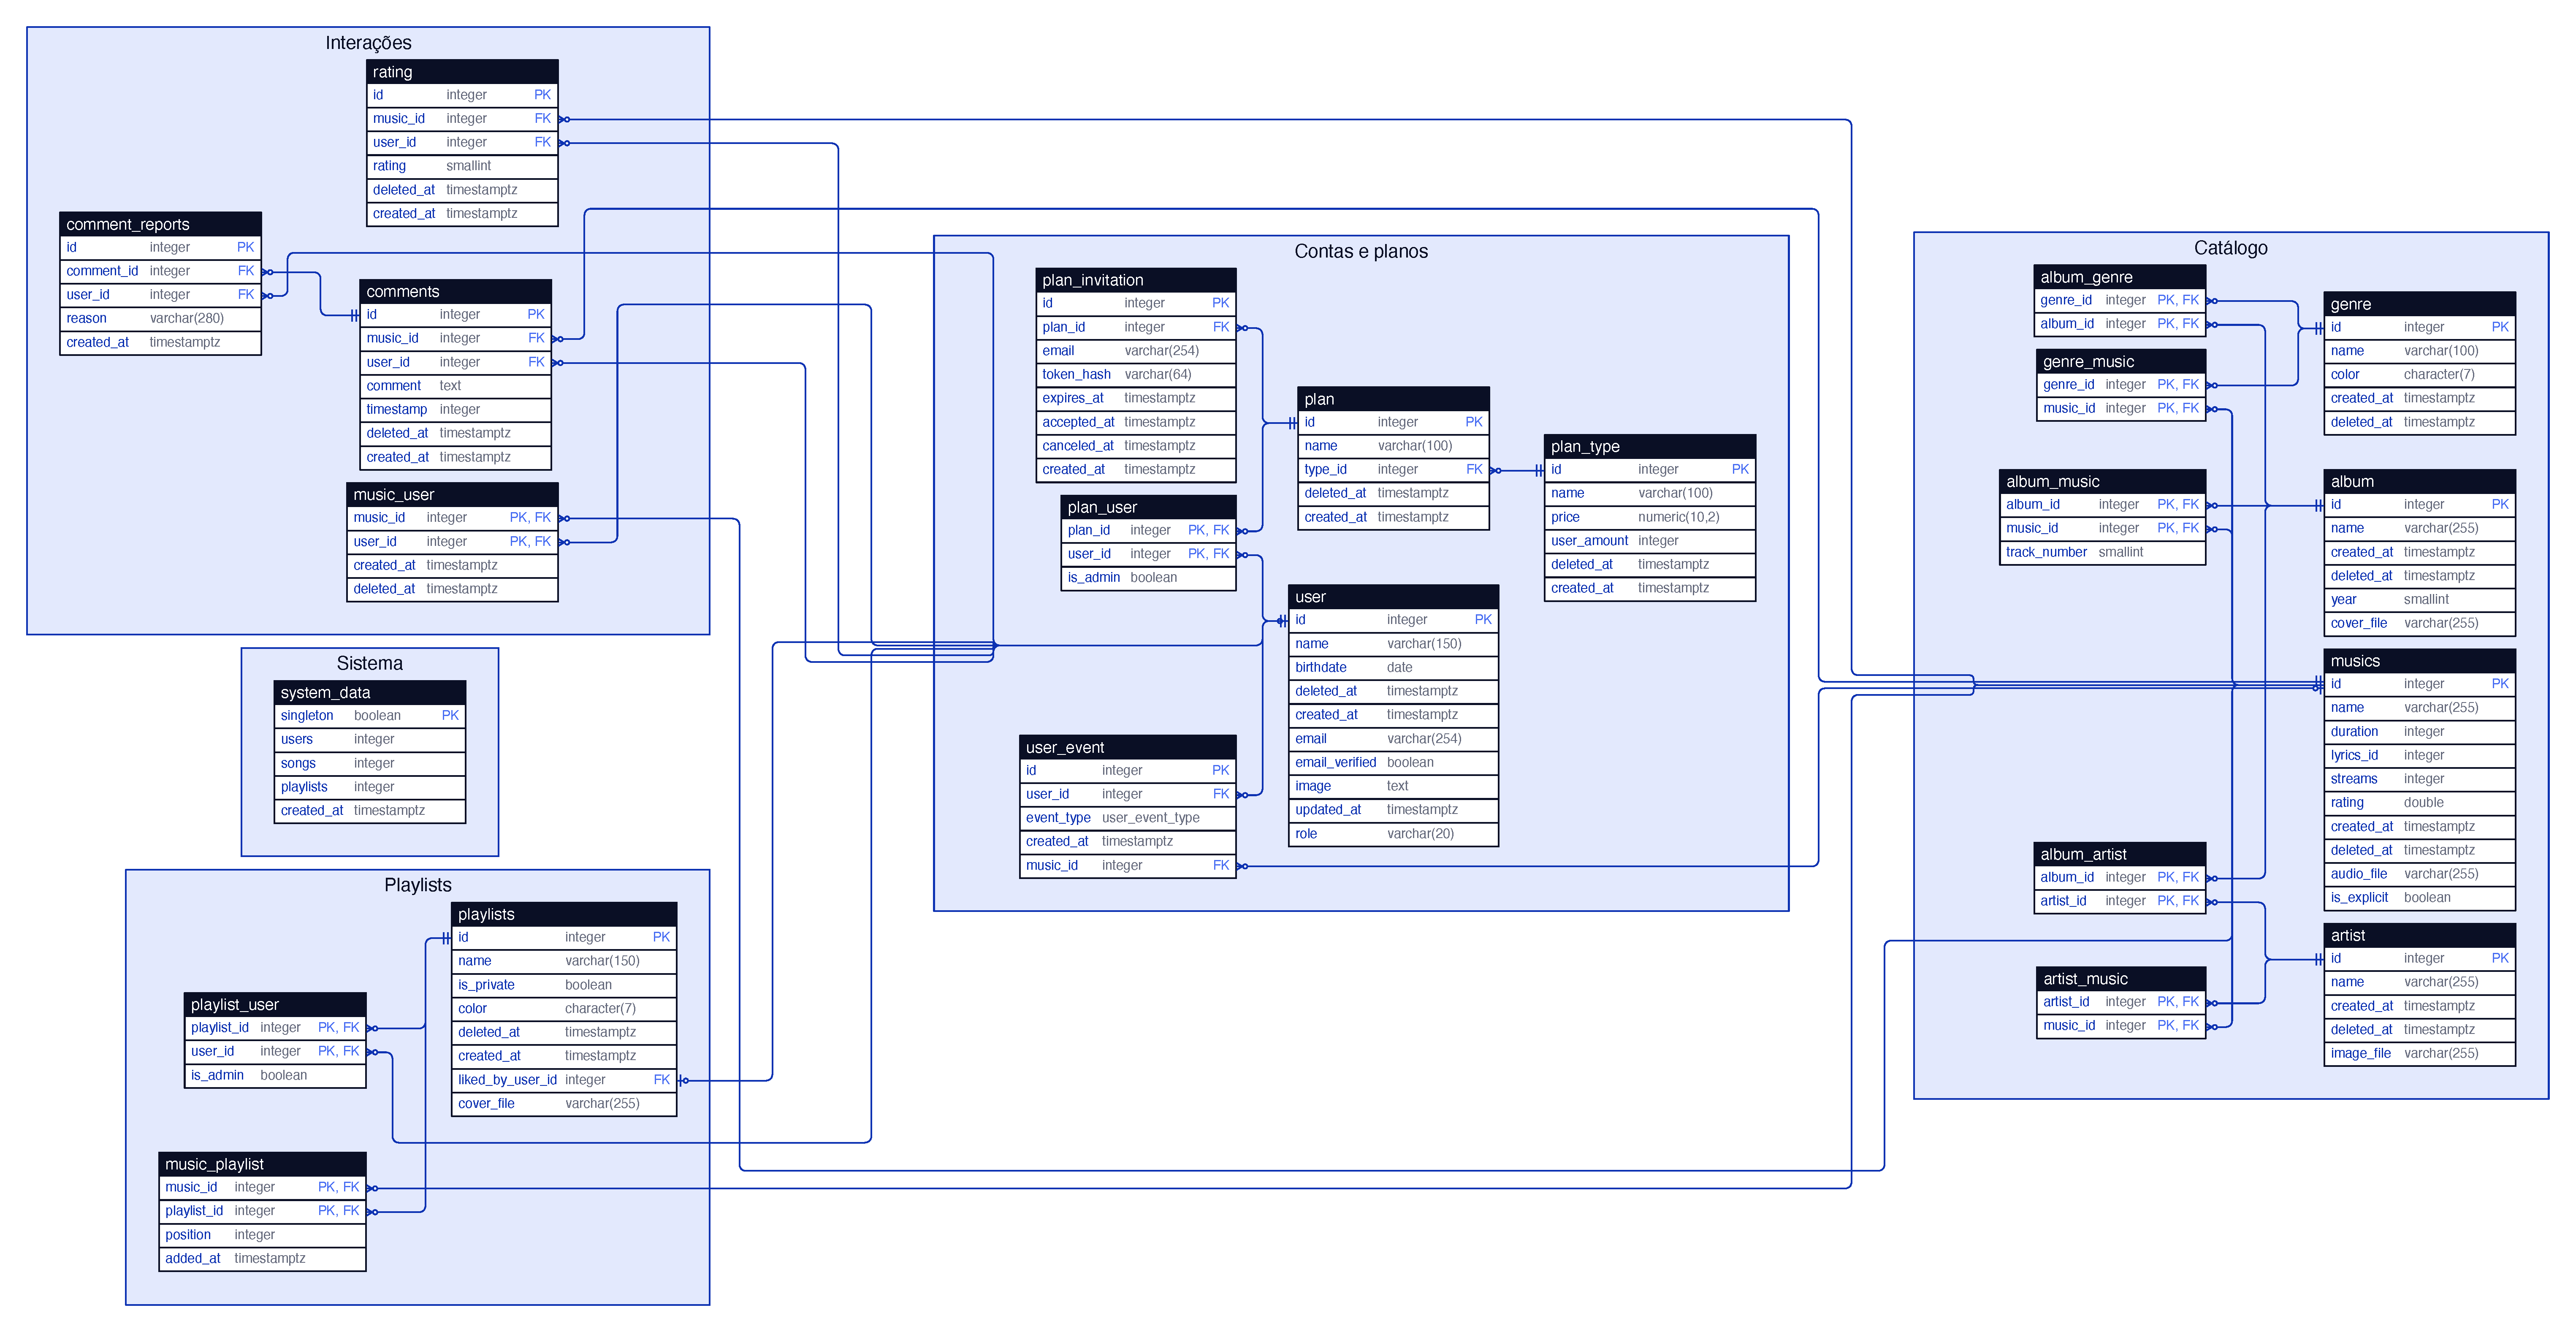
\includegraphics[width=\textwidth]{figuras/modelo-relacional.pdf}
  \caption{Modelo relacional, gerado a partir do próprio banco pelo script
    \campo{db:erd} (sem as tabelas do Better Auth)}
  \label{fig:relacional}
\end{figure}

A \cref{fig:relacional} não é desenhada à mão. O script \campo{db:erd} lê as
tabelas, colunas e chaves do catálogo do Postgres e desenha o diagrama com o
D2. O GitHub Actions o executa a cada push, então a figura sempre corresponde
ao banco.

\FloatBarrier
\subsection{Tabelas}

\begin{table}[htbp]
  \centering
  \caption{Tabelas do banco, por área}
  \label{tab:tabelas}
  \small
  \begin{tabularx}{\textwidth}{@{}L{0.6}L{0.9}L{1.5}@{}}
    \toprule
    \poliCabTabela{Área} & \poliCabTabela{Tabela} & \poliCabTabela{O que guarda} \\
    \midrule
    Contas e planos & \campo{user} & As contas; é também a tabela de usuários do Better Auth \\
     & \campo{plan\_type} & Os tipos de plano, com preço e limite de pessoas \\
     & \campo{plan} & Os planos assinados \\
     & \campo{plan\_user} & Quem está em cada plano e quem é o gestor (\campo{is\_admin}) \\
     & \campo{plan\_invitation} & Os convites do plano familiar \\
     & \campo{user\_event} & Os eventos de uso, com a música quando é uma reprodução \\
     & \campo{system\_data} & Contadores gerais do sistema, numa única linha \\
    \midrule
    Catálogo & \campo{musics} & As músicas \\
     & \campo{album}, \campo{artist}, \campo{genre} & Os álbuns, os artistas e os gêneros \\
     & \campo{album\_music} & As faixas de cada álbum, com \campo{track\_number} \\
     & \campo{artist\_music}, \campo{album\_artist} & Os artistas de cada música e de cada álbum \\
     & \campo{genre\_music}, \campo{album\_genre} & Os gêneros de cada música e de cada álbum \\
    \midrule
    Playlists & \campo{playlists} & As playlists \\
     & \campo{playlist\_user} & Os membros de cada playlist e quem a administra \\
     & \campo{music\_playlist} & As músicas de cada playlist, em ordem \\
    \midrule
    Interações & \campo{rating} & As avaliações de 1 a 5 \\
     & \campo{music\_user} & As músicas salvas por cada conta \\
     & \campo{comments} & Os comentários \\
     & \campo{comment\_reports} & As denúncias de comentários, com o motivo \\
    \midrule
    Autenticação & \campo{session} & As sessões abertas; o \campo{token} é o valor do cookie \\
     & \campo{account} & Uma linha por forma de login; com email e senha, guarda o hash \\
     & \campo{verification} & Tokens de confirmação de email e recuperação de senha \\
    \bottomrule
  \end{tabularx}
\end{table}

\FloatBarrier
\subsection{Convenções}

\begin{itemize}
  \item \textbf{Nomes} em inglês e \emph{snake\_case}. As constraints seguem o
    padrão do Prisma (\campo{<tabela>\_pkey}, \campo{<tabela>\_<coluna>\_fkey}),
    para que o \campo{schema.prisma} gerado não precise de mapeamentos.
  \item \textbf{Datas} em \campo{timestamptz}, com fuso. As tabelas registram
    \campo{created\_at} e, quando há remoção lógica, \campo{deleted\_at}. Só
    as tabelas do Better Auth têm \campo{updated\_at}, porque a biblioteca
    atualiza esses registros.
  \item \textbf{Arquivos} (áudio das músicas, capas e fotos) ficam fora do
    banco, num diretório do servidor. O banco guarda só o nome do arquivo
    (\campo{<uuid>.mp3}), para que o diretório possa mudar sem migrar dados.
  \item \textbf{Senhas e tokens} nunca são guardados em texto puro. A senha
    fica em \campo{account.password} com hash \emph{scrypt}, e o convite
    guarda só o hash SHA-256 do token do link.
\end{itemize}
